% 
% Annual Cognitive Science Conference
% Sample LaTeX Paper -- Proceedings Format
% 

% Original : Ashwin Ram (ashwin@cc.gatech.edu)       04/01/1994
% Modified : Johanna Moore (jmoore@cs.pitt.edu)      03/17/1995
% Modified : David Noelle (noelle@ucsd.edu)          03/15/1996
% Modified : Pat Langley (langley@cs.stanford.edu)   01/26/1997
% Latex2e corrections by Ramin Charles Nakisa        01/28/1997 
% Modified : Tina Eliassi-Rad (eliassi@cs.wisc.edu)  01/31/1998
% Modified : Trisha Yannuzzi (trisha@ircs.upenn.edu) 12/28/1999 (in process)
% Modified : Mary Ellen Foster (M.E.Foster@ed.ac.uk) 12/11/2000
% Modified : Ken Forbus                              01/23/2004
% Modified : Eli M. Silk (esilk@pitt.edu)            05/24/2005
% Modified : Niels Taatgen (taatgen@cmu.edu)         10/24/2006
% Modified : David Noelle (dnoelle@ucmerced.edu)     11/19/2014
% Modified : Roger Levy (rplevy@mit.edu)     12/31/2018



%% Change "letterpaper" in the following line to "a4paper" if you must.

\documentclass[10pt,letterpaper]{article}

\usepackage{cogsci}
\usepackage{color}

\cogscifinalcopy % Uncomment this line for the final submission 


\usepackage{pslatex}
\usepackage{graphicx}
\usepackage{amsmath}
\usepackage{apacite}
\usepackage{float} % Roger Levy added this and changed figure/table
                   % placement to [H] for conformity to Word template,
                   % though floating tables and figures to top is
                   % still generally recommended!

%\usepackage[none]{hyphenat} % Sometimes it can be useful to turn off
%hyphenation for purposes such as spell checking of the resulting
%PDF.  Uncomment this block to turn off hyphenation.


%\setlength\titlebox{4.5cm}
% You can expand the titlebox if you need extra space
% to show all the authors. Please do not make the titlebox
% smaller than 4.5cm (the original size).
%%If you do, we reserve the right to require you to change it back in
%%the camera-ready version, which could interfere with the timely
%%appearance of your paper in the Proceedings.


\title{One and known: Incidental probability judgments from very few samples}
 
\author{{\large \bf Ishan Singhal\textsuperscript{1,2} (ishan20@iitk.ac.in), Narayanan Srinivasan\textsuperscript{1,2}  (nsrini@iitk.ac.in)} \\
  \textsuperscript{1}Department of Cognitive Science, IIT Kanpur \\
   Kanpur 208016 India\\
  \textsuperscript{2}Centre of Behavioural and Cognitive Science, University of Allahabad\\
  Allahabad 211002 India
  \AND {\large \bf Nisheeth Srivastava (nsrivast@iitk.ac.in)} \\
  Department of Computer Science, IIT Kanpur\\
  Kanpur 208016 India}

\begin{document}

\maketitle


\begin{abstract}
We test whether people are able to reason based on incidentally acquired probabilistic and context-specific magnitude information. We manipulated variance of values drawn from two normal distributions as participants perform an unrelated counting task. Our results show that people do learn category-specific information incidentally, and that the pattern of their judgments is broadly consistent with normative Bayesian reasoning at the cohort level, but with large individual-level variability. We find that this variability is explained well by a frugal memory sampling approximation; observer models making this assumption explain approximately 70\% of the variation in participants' responses. We also find that behavior while judging easily discriminable categories is  consistent with a model observer drawing fewer samples from memory,  while behavior while judging less discriminable categories is better fit by models drawing more samples from memory. Thus, our model-based analysis additionally reveals resource-rationality in memory sampling.

%\keywords{Bayesian cognitive science; value; mental representations}

\end{abstract}

\section{Introduction}

Statistical inference offers a compelling normative criterion for human judgments during perception and action. Strong evidence of probabilistic reasoning is available for perceptual judgments~\cite{ernst2002humans} and sensorimotor control~\cite{kording2004bayesian}, wherein human performance in cue integration tasks has been shown to closely follow normative Bayesian principles~\cite{pouget2013probabilistic}. There is also some evidence suggesting how Bayesian updates for such settings could be carried out by populations of neurons~\cite{ma2006bayesian}.

Similar normative claims have also been advanced for human cognition, supported by evidence from a a wide variety of cognitive tasks~\cite{oaksford2007bayesian, tenenbaum2011grow}.
However, critics contend that Bayesian analysis offers too many degrees of freedom to the analyst in the design of appropriate priors and likelihood, such that empirical fits with data can often be attributed to environmental and psychological properties embedded in the design of these entities~\cite{jones2011bayesian}. 

Properties of the environment and biophysical embodiment can strongly constrain the nature of priors in perceptual and motor control tasks and some language-related cognitive tasks. However, it is harder to produce such constraints for cognitive tasks wherein embodiment is weakly involved and environmental statistics are variable. For instance, to accept ~\citeA{griffiths2006optimal}'s contention that humans are Bayes-optimal in making commonplace probability judgments, we must believe that people {\em incidentally} keep track of the distribution of a large variety of real-world events. Similarly, to accept the explanation for risk aversion offered in ~\citeA{stewart2006decision}'s decision-by-sampling theory, we must believe that people incidentally track the distribution of money magnitudes. 

While there is some evidence that people track incidental frequencies well~\cite{hz84}, more direct tests of incidental distribution learning have been discouraging~\cite{sailor2005memory, tvp17}. Given 180 samples from a bimodal distribution of stimulus locations, for example, humans are effectively random in trying to reproduce the distribution again via sampling~\cite{tvp17}. 

In summary, while there is considerable evidence to support the case that humans reason probabilistically given an understanding of the appropriate generative model of the world, it is less clear how they are {\em incidentally} able to acquire and update these generative models and apply them to novel situations. In this study, we tested peoples' ability to {\em incidentally} learn about context-specific distributions of magnitudes, and reason with them retrospectively. We analyzed participants' behavior with observer models fitted to observations that participants saw during {\em incidental} learning to characterize the nature of mental representations used in this retrospective probabilistic reasoning task.

\section{Experiment}

%We tested the observer model's predictions by manipulating variance of the sequentially observed value distribution between subjects.

We implemented our test for {\em incidental} learning of context-specific probability distributions as a game where participants were asked to assume the role of financial auditors and check restaurant bills for correct total and tip values (tip values had to be less than 10\% of the sum of the items' cost). This simple arithmetic task allowed us to expose participants to the values of the items on the bills, ensuring they paid attention to them while remaining naive to the true purpose of the experiment. 
	
\begin{figure}[htbp]
	\centering
	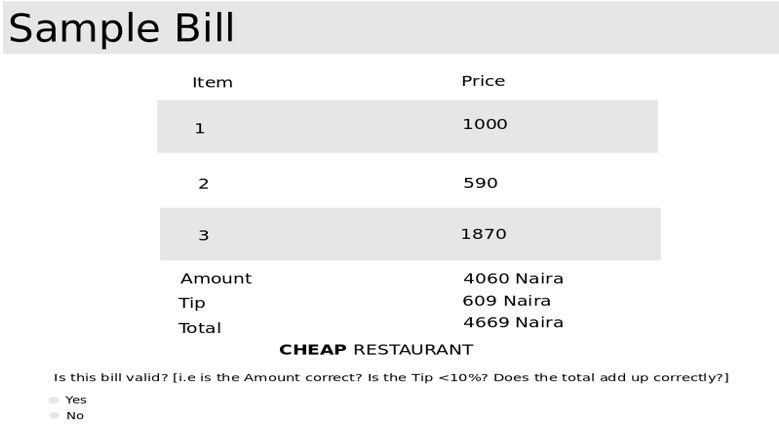
\includegraphics[width=0.45\textwidth]{results/sample-bill.JPG}
	\caption{Sample bill presented in the training phase of the experiment.}
	\label{fig:design}
\end{figure}

There were two phases in the experiment: {\em training} and {\em testing}. During training, participants were shown a number of restaurant bills (see sample bill in Figure \ref{fig:design}). Each bill had three items listed with money values. These bills were explicitly identified as being from either “cheap” or “expensive” restaurants. Restaurant category had no bearing on the auditing task. The items were denominated in a fictional foreign currency to reduce the influence of participants' prior knowledge of money magnitudes in this context. 

The training phase was meant to instantiate the value distributions $p(money|context)$ and the probability of context occurrence $p(context)$ in participants. During the testing phase, on every trial, participants were presented with an item alongside its price, and asked to assess how likely it was that the item came from an expensive restaurant, thus asking them to express $p(context|money)$.

%We tested whether the variance of the likelihood function would alter participants' posterior responses. The Bayesian observer model predicts that increasing variance would lead to increased confusion in classifying and discriminating between two value distributions~\cite{srivastava2014magnitude}.

\subsection{Participants}
The study protocol was reviewed and approved by an IRB. The study was conducted using a web interface. A total of 91 (mean age = 25.1years, females = 44) participants completed the experiment. Seven participants with poor performance (less than 80\% accuracy) in the training phase were excluded from the study. Unmotivated participants (8 such) who responded with identical responses for all the test phase problems were also excluded from analysis resulting in 76 participants. {\em A priori} sample size calculated was for 72 participants (Cohen’s f = 0.4, power = 0.85). The hypothesis, sample size and analysis plan were formally preregistered (link concealed to preserve anonymity during peer review). 

\subsection{Stimuli}

In the training phase of the experiment, we showed participants values drawn from two normal distributions. Values from each distribution were shown as bills from restaurants with two category labels, “cheap” and “expensive” (See Fig.1.). We manipulated the variance (low, medium, high) of these distributions between participants with number of participants being 25, 26 and 25 respectively. Cheap and expensive labels each had their own distribution and we scaled the variance by the mean (fixed means for cheap = 1600 and expensive = 2900, scaling variance factors: low = 0.25, medium = 0.5 and high = 0.7).  

%\begin{table}[]
%    \centering
%    \begin{tabular}{c|c|c|c}
%    \hline
%    Experiment & Mean (cheap, expensive) & Mean scaled variance factor & Skewness\\
%    \hline
%         1 & 1600, 2900 & 0.25, 0.5, 0.7 & 0  \\
%         2 & 1600, 2900 & 0.5, & 0\\
%         3 & 1000, 1600 & 0.5 & 4,-4; -4,4\\
%    \end{tabular}
%    \caption{Mean, variance and skewness values of the distributions used to generate cheap and expensive restaurant item values}
%    \label{tab:my_label}
%\end{table}

\subsection{Procedure}
	
\subsubsection{Training Phase}
	
Participants were randomly assigned to one of three variance groups. Thus, a participant could see values drawn in the training phase from either a distribution with low, medium or high variance. The means of these value distributions (for cheap and expensive restaurants) were kept constant across all participants. We asked each participant to audit 20 bills as part of the experiment, with each bill containing three money values sampled from the condition-specific distribution. There were 10 bills each (30 samples; 3 x10) for 'cheap' and 'expensive' restaurant bills. We provided feedback (correct/incorrect) for their responses on each bill as an attention check. Participants who performed poorly on the arithmetic task (accuracy less than 80\%) were eliminated from analysis. 

\subsubsection{Testing Phase}
During the training phase conducted earlier, participants were unaware that they would be tested on the values given in the bills, i.e. they were tested retrospectively. In this phase, participants were presented with 40 individual items, each with a certain value. They were asked to indicate how likely it is that these items were drawn from an expensive restaurant on a seven point Likert scale. All participants were tested on values generated from the same distribution with variance factor 0.5. This allowed us to compare responses between the three groups and investigate whether their priors for “expensive” and “cheap” restaurants was biased by the variance of the distribution they trained on. 

\subsection{Analysis and Results}

We fit each participant's responses from the testing phase with  a psychometric function,$\gamma +\frac{\lambda - \gamma }{1 + (\frac{x}{c})^{\beta}}$ using the curve fitting toolbox in MATLAB. Here $\gamma$ was the lower asymptote of the psychometric curve, $\lambda$ was the upper asymptote, \textit{c} was the inflexion point of the curve and $\beta$ was the steepness or the slope of the curve. To fit the curves, we converted Likert ratings to probability judgements by using a recently validated mapping of verbal labels to assigned probabilities \cite{hancock2020quantifying}\footnote{Specifically, we mapped our 7-point Likert scale with labels [very unlikely, unlikely, somewhat unlikely, undecided, somewhat likely, likely, very likely] to the numbers [0.05, 0.20, 0.35, 0.50, 0.60, 0.70, 0.90] respectively.}.

%The average $R^2$ value for the fit was 0.81. [for which VF condition?]

%\begin{table}[htb]
%\caption{The table lists our conversion from Likert ratings to assigned probabilities.}
%\label{tab:my-table}
%\resizebox{\columnwidth}{!}{%
%\begin{tabular}{|l|l|}
%\hline
%Likert Ratings        & Assigned Probability \\ \hline
%1 = Very Unlikely     & 0.05                 \\ \hline
%2 = Unlikely          & 0.2                  \\ \hline
%3 = Somewhat Unlikely & 0.35                 \\ \hline
%4 = Undecided         & 0.5                  \\ \hline
%5 = Somewhat Likely   & 0.6                  \\ \hline
%6 = Likely            & 0.7                  \\ \hline
%7 = Very Likely       & 0.9                  \\ \hline
%\end{tabular}%
%}
%\end{table}

We ran a between subject Bayesian ANOVA with three conditions of variance (high, medium, low) for all four parameters in JASP (0.13.1.0) with a default cauchy prior. The alternate hypothesis that variance conditions would change the slopes ($\beta$) of the fitted curves had strong evidence (\textit{BF\textsubscript{10}} = 7771000, error\% = 0.001). Our Post-hoc tests for the same showed that the slopes of the fitted curves for participants in the low variance group were more likely to be higher than the those in the medium (posterior odds = 66391,  \textit{BF\textsubscript{10U}} = 113025) and high variance group (posterior odds = 1054,  \textit{BF\textsubscript{10U}} = 1795), while we found no evidence either way for difference in slopes for medium and high variance groups (posterior odds = 1.3,  \textit{BF\textsubscript{10U}} = 2.28). See figure 2 for the slope differences between the groups. There was weak to moderate evidence for the null for inflexion point (\textit{BF} = 3.39) and lower bound (\textit{BF} = 6.26), and inconclusive evidence (\textit{BF} = 0.53) for the upper bound.


\begin{figure}[h!]
    \centering
    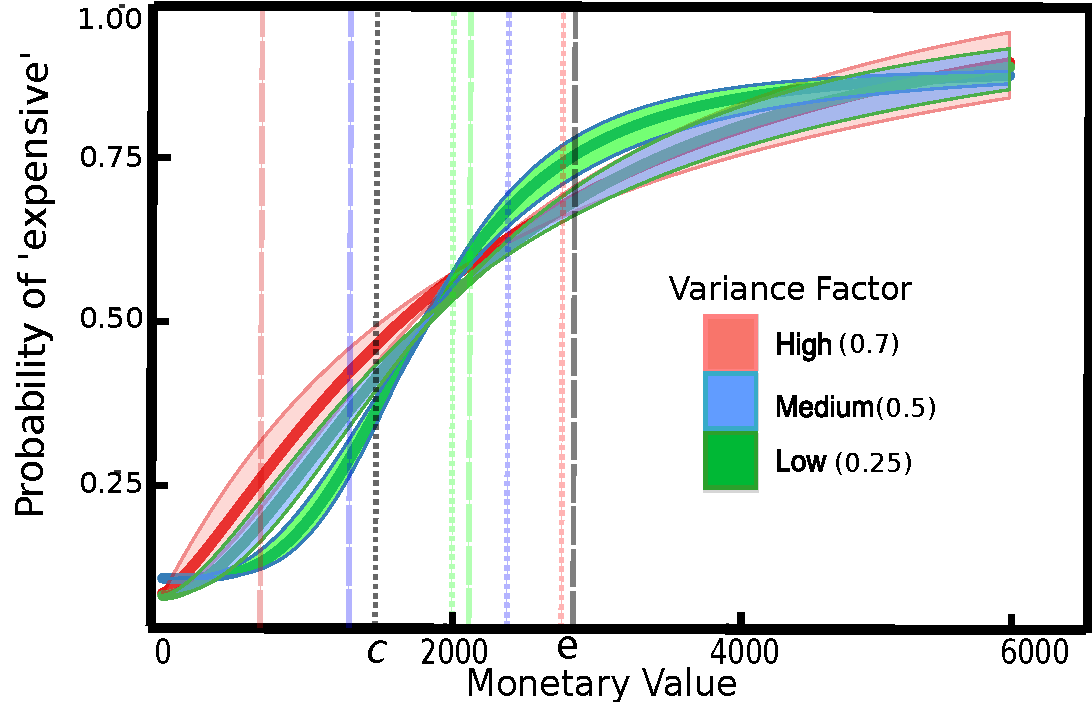
\includegraphics[width=0.45\textwidth]{results/slope.pdf}
    \caption{Psychometric function fit using averages of parameters estimated for participants for all three conditions. Shading indicates 95\% CI for slope parameter estimates. Dashed and dotted lines indicate mean and SD (one line per condition) for the three 'expensive' and 'cheap' distributions respectively. The color for the shading and dotted lines indicates the three variance conditions.}
    \label{fig:my_label}
\end{figure}

\subsection{Discussion}

Psychometric analysis of the data supports the hypothesis that the spread of the distribution of numerical observations during training will affect the posterior probability of category judgments elicited during the surprise testing phase. While our experiment is set up to determine whether people can reason with numerical quantities acquired via experience in a Bayesian manner, it can also be viewed as a categorization task. We show observers instances of two categories - cheap and expensive restaurants, and then (stochastically) ask them to classify new instances into one of them. The fact that greater within-category variance makes categorization more challenging is well-documented for both supervised~\cite{alfonso2002makes} and unsupervised category learning~\cite{kloos2008s}. It is also modeled quite well by classic computational models of categorization~\cite{fried1984induction, anderson1991adaptive}. 

However, {\em incidental} category learning of the nature we find here has not been documented previously. Participants in our experiment were asked to audit bills for totalling mistakes during training, and were not given feedback about their responses during testing nor did they know that a testing phase would follow. Given the retrospective nature of the design, participants did not know that they had to learn or memorize the values for different category labels. Studies showing successful unsupervised learning of categories tend to use highly separated categories, and any increase in within category variance tends to make category learning very hard even given 100s of training trials~\cite{ell2012impact}. Viewed in this light, the fact that people are able to {\em incidentally} learn categories in this task from 30 examples per category is significant\footnote{See Experiment 4 in ~\citeA{fried1984induction} for a historical example of surprising incidental learning of category structure.}.Our primary interest in this experiment is to characterize the extent to which participants' behavior can be explained by a Bayesian observer model, which is described in the next section. 

\section{Ideal observer model}

Our observer model is straightforward. From the behavioral results, it is evident that people are able to significantly track the joint distribution $p(K,Y)$, where $K$ is a discrete random variable indexing restaurant category and $Y$ is a continuous random variable indexing natural numbers corresponding to money magnitudes in our experiment. In the testing phase, participants are asked to express $p_{K|Y}(k|y)$, the conditional probability of $k$, given any particular numerical magnitude $y$.  

The ideal observer will construct this quantity using Bayes rule as follows,
\begin{equation}
    p_{K|Y}(k|y) = \frac{p_K(k)f_{Y|K}(y|k)}{f_Y(y)},
    \label{eqn:main}
\end{equation}

where $f_Y$ is the pdf of a mixture of the two components, and $f_{Y|K}$ is a single component's pdf. To parameterize this model, we model $p_K$ as a Bernoulli trial $p_K(\theta)$, both $p_{Y|K}$ as Gaussian distributions $f_{Y|K}(y|\mu^k, (\tau^k)^{-1})$, and $p_Y$ as a mixture of these Gaussians weighted by the Bernoulli distribution. The distribution $p_{K|Y}$ remains without a concise parametric specification, and is simply readout in tabular form. 

%Similarly, observers will track the category-specific magnitude distribution,
%\begin{equation}
%    f_{Y|K}(y|k) = \frac{f_Y(y)p_{K|Y}(k|y)}{p_K(k)},
%\end{equation}

%and the relevant marginals can be computed over these conditionals,

%\begin{align}
%    f_Y(y) &= \sum_{k'}p_K(k')f_{Y|K}(y|k') \label{eqn:mixture} \\
%    p_K(k) &= \int_{y'}f_Y(y')p_{K|Y}(k|y')dy'
%\end{align}


\begin{figure}
    \centering
    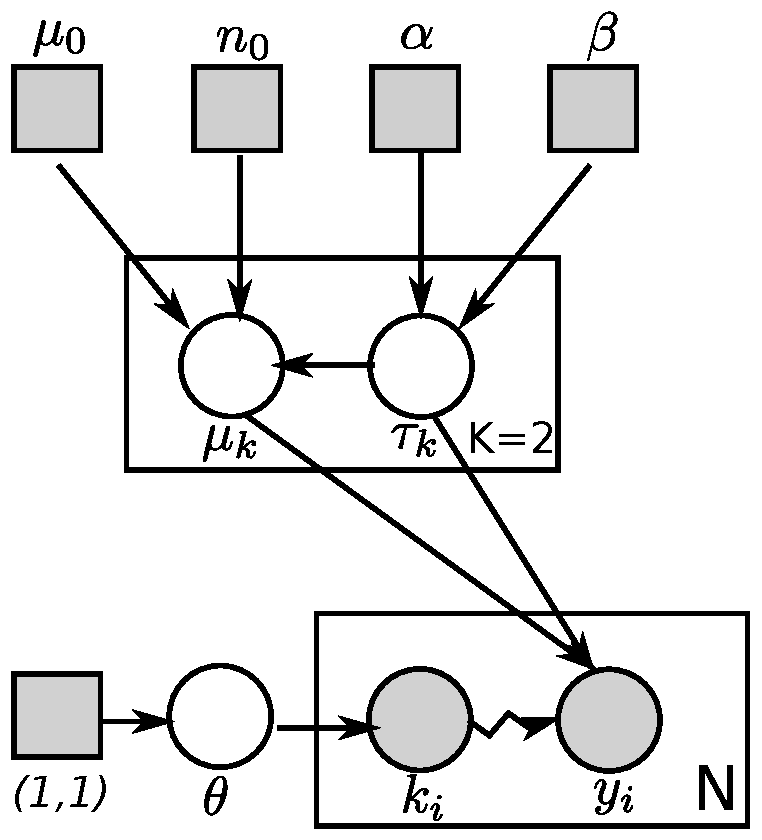
\includegraphics[width=0.4\textwidth]{results/model.pdf}
    \caption{Generative model for experimental task in plate notation.}
    \label{fig:model}
\end{figure}

We assume that people enter the experiment with some Gaussian $f_{Y|K}$ and $f_Y$, and update these as they go along in the experiment. We also assume they start with some Bernoulli $p_K$ and an improper uniform prior of 0.5 on the positive half-line for $p_{K|Y}$. These initial conditions are specified by means of hyper-parameters, following a generative model very similar, but slightly different from a Bayesian Gaussian mixture model~\cite{bishop2006pattern}, as illustrated in Figure~\ref{fig:model}. The key difference is that the mixture component identity is co-observed alongside numerical magnitudes on each observation rather than being a latent variable. 

When a new observation $\{y_{obs}, k_{obs}\}$ appears, $y_{obs}$ updates the $p_{Y|K}$ distribution corresponding to $K = k_{obs}$, and $k_{obs}$ updates the $p_k$ distribution. We model the $k$ update as a Bernoulli update with a Bayes estimator using an uninformative $Beta(1,1)$ prior. 

%This yields the update

%\begin{equation}
%    \theta \leftarrow \frac{r + 1}{n + 2},
%    \label{eqn:bern}
%\end{equation}
%where $r$ is the number of occurrences of category 'expensive' out of $n$ total observations.

We model the $y|k$ update as sequential inference about a Gaussian with unknown mean and precision using a normal-inverse-Gamma conjugate prior~\cite{murphy2007conjugate}. The ideal observer begins learning by updating hyperparameters $\theta$ for $p_K$ and $\{\alpha, \beta, \mu_0, n_0\}$ for $f_{Y|K}$. Then it updates the marginal $f_Y$ and finally uses Equation~\ref{eqn:main} to calculate $p_{K|Y}$. 

%For each Gaussian component, this inference follows the generative model 
%\begin{align}
%    y_i|\mu, \tau &\sim N(\mu, \tau), \nonumber \\
%    \mu | \tau &\sim N(\mu_0, n_0\tau), \nonumber \\
%    \tau &\sim Ga(\alpha, \beta), \nonumber
%\end{align}
%yielding analytic parameter updates on observing $y_i$.

%\begin{align}
%    \alpha &\leftarrow \alpha + \frac{n}{2}, \nonumber \\
%    \beta &\leftarrow \beta + \frac{1}{2}\sum{(y_i - \bar{y})^2 + \frac{nn_0}{2(n+n_0)}(\bar{y} - \mu_0)^2},  \nonumber \\
%    \mu_0 &\leftarrow \frac{n\tau}{n\tau + n_0\tau} \bar{y} + \frac{n_0\tau}{n\tau + %n_0\tau} \mu_0  \nonumber \\
%    n_0 &\leftarrow n + n_0 \label{eqn:gauss}
%\end{align}

%\begin{figure}[h!]
%    \centering
%    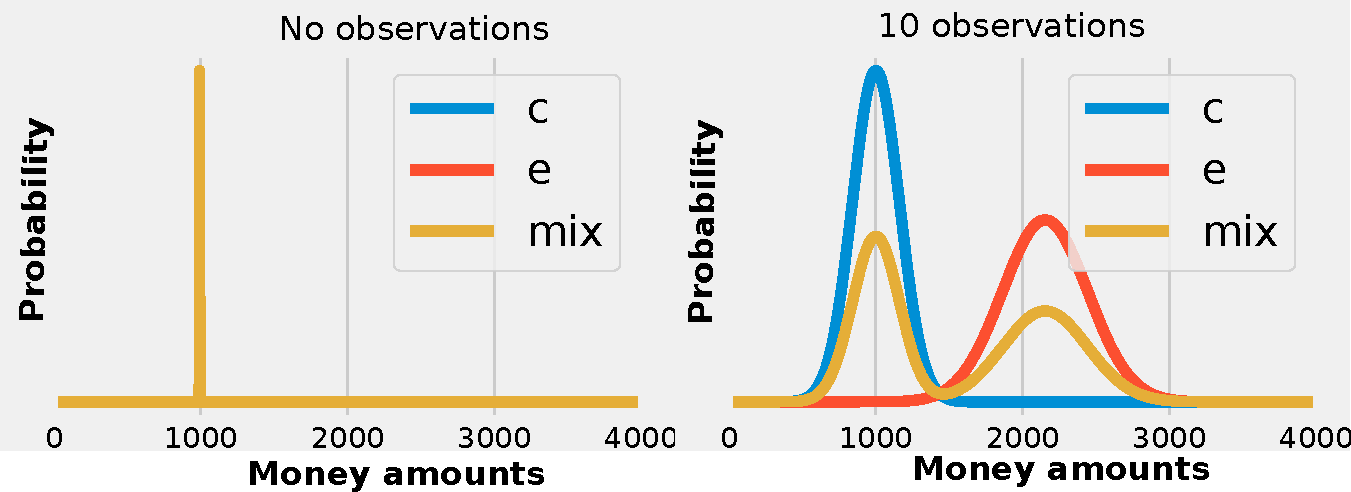
\includegraphics[width=0.45\textwidth]{results/component_update.pdf}
%    \caption{Illustration of sequential Bayesian update of mixture components (left) %having seen no magnitude samples, and (b) having seen five magnitude samples per category.}
%    \label{fig:components}
%\end{figure}

%The ideal observer begins learning by updating the parameter for $p_K$ using Equation~\ref{eqn:bern} and the parameters for $f_{Y|K}$ for the correct mixture component using Equations~\ref{eqn:gauss} given above, as illustrated in Figure~\ref{fig:components}. Then it updates the marginal $f_Y$ using Equation~\ref{eqn:mixture}, and finally uses Equation~\ref{eqn:main} to calculate $p_{K|Y}$. 
%The ideal observer begins learning by updating hyperparameters $\theta$ for $p_K$ and $\{\alpha, \beta, \mu_0, n_0\}$ for $f_{Y|K}$. Then it updates the marginal $f_Y$ and finally uses Equation~\ref{eqn:main} to calculate $p_{K|Y}$. 

%\begin{figure}
%    \centering
%    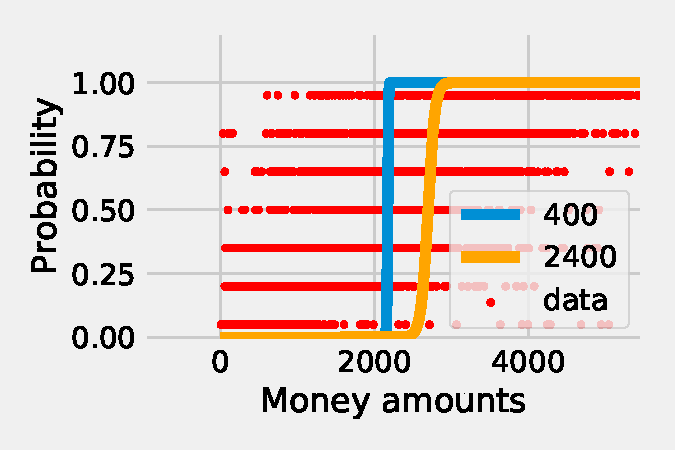
\includegraphics[width=0.45\textwidth]{results/sim_slope.pdf}
%    \caption{Observer model predictions for observations made from normal distributions with means identical to experimental means used and three different variance values for the generating distributions.}
%    \label{fig:sim_slope}
%\end{figure}

%Before attempting to fit data to this model, we first conduct simulations to qualitatively validate the basic prediction of greater confusability for category judgments given exposure to training data with greater variance. Figure~\ref{fig:sim_slope} shows that the model does support this prediction. When trained with 60 observations of money amounts, as in our experiment, the model's posterior probability $p_{K|Y}$ shows a shallower slope when trained with observations emitted from component distributions with high variance than with low variance. 

%However, notice that neither distribution, obtained from the lowest and highest variances used in the actual experiment, shows a particularly close fit to the actual data (compare the slopes of the logistic curve in Figure~\ref{fig:sim_slope} with the slopes estimated from the data in Figure~\ref{fig:my_label}). 

\section{Model-based Analysis}

As~\citeA{jones2011bayesian} point out, it is important to justify the psychological assumptions embedded in Bayesian models to truly bring them into alignment with reality. In the context of our task, the ideal observer assumes that, when asked to express a probability judgment about category membership, a human constructs this belief by retrieving all 60 training samples from memory to update their generative model. Therefore, for our model-based analysis, we also consider two frugal alternatives to this baseline observer model,
\begin{enumerate}
    \item inspired by prototype models of categorization~\cite{fried1984induction, minda2001prototypes}, we consider a {\em prototype} observer model which assumes that people retrieve the mean of category distributions observed during training phase, and update an abstract generative model of world situations like the given task with just this pair of mental observations while constructing probability judgments in our task. 
    \item inspired by recent Bayesian sampling proposals~\cite{sanborn2016bayesian, zhu2020bayesian}, we consider a memory {\em sampling} extension of the prototype observer model, which assumes that people either encode or retrieve a subset of training phase observations to construct prototypes, which are then used to construct probability judgments as in the prototype observer model. 
\end{enumerate}

We first analyzed all three models' ability to account for our data with a single set of pooled hyperparameters estimated across all participants. We fit the observer models to data by giving it sequential access to 60 original observations seen by each participant during their training phase in each of the three conditions and then using these three condition-specific trained models to predict posterior probabilities for the 40 observations seen by participants during the test phase. We obtained max likelihood estimates for all parameters, and calculated BIC scores for all models' predictions compared with our data. Since the posteriors emitted by the sampling observers vary because of the stochastic nature of their likelihoods, we report median BIC scores obtained across 100 simulations each for these two models. 

\begin{table}[]
    \centering
    \begin{tabular}{|c|c|c|c|}
    \hline
         Model/VF & 0.25 & 0.5 & 0.7 \\
         \hline
         Ideal & -3352 & -3241 & -3093 \\
         Prototype & -3057 & -3498 & -3476 \\
         Sampling & -3204 (5) & -3637 (5) & -3614 (6) \\
         \hline 
    \end{tabular}
    \caption{BIC scores for observer models fit condition-wise. SEM across multiple runs reported in brackets. All results rounded to integers.}
    \label{tab:bic}
\end{table}

Both the alternative models are clearly superior to the ideal observer across high variance training conditions. Interestingly, overall the sampling observer explains the data better than the ideal observer, as measured by BIC. Thus, in an empirical sense at least, it is evident that observers that compress incoming magnitude information into category prototype representations are better models for participants' judgments in our task than fully Bayesian observers with perfectly individuated memory of exemplars. The high correspondence between the prototype model and our data (absolute goodness-of-fit $RMSE=0.15$ across all three conditions) suggests that human observers possess a normatively appropriate generative model applicable for the task we asked them to do retrospectively and invert it to obtain situation-specific probabilistic judgments by drawing a few samples of past observations from memory.  

We next considered model fits with hyperparameters estimated at the per participant level. Figure~\ref{fig:Figure_4}A-B summarizes goodness-of-fit for the ideal observer making predictions on the observations seen by each participant during the test phase. Panel A plots the model's predicted posterior distribution $p_{K|Y}$ against one participant's probabilistic responses. Panel B summarizes median goodness-of-fit, quantified using adjusted $R^2$ obtained for participants, training the model using the same values as observed during the training phase by each participant in a given condition, and setting hyperparameters for each participant using max likelihood estimation. The results suggest that the ideal observer models variability in individuals' responses for easier discrimination judgments reasonably, but is increasingly less effective in modeling variability in responses for harder discriminations. 

\begin{figure}[h!]
    \centering
    \includegraphics[width=0.4\textwidth]{results/Figure_4.png}
    \caption{Ideal observer model (A) fit to one participant's data, and (B) median goodness-of-fit measured across all participants by condition. Median goodness of fit for a (C) prototype observer model and a (D) sampling observer model. Error bars represents $\pm 1$ s.e.m.} 
    \label{fig:Figure_4}
\end{figure}

Figure~\ref{fig:Figure_4}C-D summarizes goodness-of-fit for these two observer models. Overall, they afford better descriptions of individuals' data than the ideal observer model, because of the extra modeling flexibility afforded them by the introduction of two (prototype model - both prototype values) and one (sampling model - sample count) additional parameters. 

An additional analysis of the sampling observer model affords additional insight into peoples' behavior. Figure \ref{fig:meta_sampling} plots adjusted $R^2$ values across all participants achieved by sampling models restricted to drawing a fixed number of observations from memory per category. The value reported in the graph is the median of 100 runs of the model for each sample count level to account for the stochasticity of memory sampling. We see that the model's ability to explain behavioral variation for participants exposed to high variance training distributions continues to improve with the number of additional samples permitted. However, interestingly, drawing as few as one to two samples per category is already sufficient for the sampling observer model to explain more than 60\% of the variance in peoples' behavior if they were assigned to the low variance training condition.   


\begin{figure}[h!]
    \centering
    \includegraphics[width=0.4\textwidth]{results/meta_sampling.pdf}
    \caption{Median sampling observer model $R^2$ measured across 100 iterations each for different counts of observations sampled. Iteration $R^2$ value is calculated as the average $R^2$ of models with that sample count fit to each participants' data. Error bars show average 1 s.e.m. across iterations.}
    \label{fig:meta_sampling}
\end{figure}

The general trend seen in Figure~\ref{fig:meta_sampling} suggests that people might be constructing prototypes using fewer samples from memory for categories that are less confusable, and more samples for categories that are more confusable. This pattern is consistent with people performing resource-rational memory sampling - drawing fewer samples from memory to construct prototypes needed to discriminate easily discriminable categories, and drawing more samples to construct prototypes needed to discriminate less discriminable categories. Resource-rational meta-reasoning has several attractive theoretical properties~\cite{griffiths2015rational}, but opinion remains divided on the extent to which such resource-rationality is simply a metaphor to add greater flexibility to Bayesian models~\cite{rahnev2020resource}, or whether it can be shown to have stronger ontic commitments~\cite{griffiths2015rational}. The pattern of meta-reasoning in Figure~\ref{fig:meta_sampling} supports the consideration of sampling as a concrete operationalization of resource-rationality for Bayesian models of cognition~\cite{srivastava2014frugal, sanborn2016bayesian}. 

% would be a stronger conclusion if we included the analysis in the paragraph below.

%This sampling could be occurring at the time the categories are encoded, or at the time of retrieval. To differentiate these two possibilities, we conducted one final analysis - counting the number of times participants responded with non-contiguous Likert responses to values within the typical just noticeable difference ($jnd = 1.08$) range for monetary valuations of this scale~\cite{dziewulski2016eliciting}. If sampling occurs at encoding, then we expect no such occurrences in the data. Instead, we find that the median participant emits such non-contiguous responses on 6 out of their total 40 elicitations (M=7.95, SD=7.98), with 80\% of participants making at least one such response. This observation supports the case for a significant role for memory sampling at the time of retrieval.     


\section{General Discussion}
We make three contributions in this paper. One, we present empirical evidence of incidental supervised category learning from very few observations, consistent with a long-standing assumption in Bayesian cognitive science that people intuitively even when not explicitly motivated store important statistical information about events in the world~\cite{griffiths2006optimal, stewart2006decision}. Two, we demonstrate using computational modelling, that humans' behavior in tests of incidental category learning are consistent with the behavior of a Bayesian observer that samples a subset of event observations from memory to construct probability judgments~\cite{srivastava2014frugal, zhu2020bayesian}. Three, we find that behavior while judging easily discriminable categories is consistent with a model observer drawing fewer samples from memory, while behavior while judging less discriminable categories is better fit by models drawing more samples. These observations are consistent with theoretical expectations of resource-rationality in memory sampling~\cite{griffiths2015rational, sanborn2016bayesian}.

Our work also demonstrates quite clearly that, whether people are able to incidentally learn distributions corresponding to real-world situations~\cite{hz84} or not~\cite{tvp17}, they can certainly learn enough about them well enough from as few as one sample per distribution to reason probabilistically about them, as presupposed by earlier work~\cite{griffiths2006optimal, stewart2006decision}. Interestingly, the prototype observer model shows excellent empirical fits with data across our three variance manipulations, even though the model itself gains no access to variance information. In short, incidental probability judgments are consistent with a `one-and-known' sampling heuristic supporting peoples' probabilistic causal inference. 

Probabilistic accounts of cognition are sometimes questioned on grounds of neurobiological plausibility. Probabilistic population codes can potentially encode and enable reasoning over distributions corresponding to invariant or slow-changing priors and well-structured likelihoods~\cite{ma2006bayesian}. It is possible to model important elements of perceptual and motor tasks using such distributions, but not for cognitive tasks of the nature we consider in this paper. Flexible probabilistic reasoning in everyday cognition appears to require operations incongruent with the extent to which and timescales on which synaptic weights can change as a function of experience~\cite{malinow1988persistent}. Our results  offer a possible resolution for this problem - sampling a small number of observations from memory, is sufficient to tune a generic situation model, potentially learned over long experience, into expressing probabilistic judgments that closely match human behavior. 


%We note that this empirically demonstrated resolution is also consistent with theoretical proposals arguing for hierarchical predictive inference as an important organizing principle for the brain~\cite{friston2009free, clark2015surfing}.

Due to the key role played by the observer's possession of the correct generative model in explaining behavior with very little further learning, this work also amplifies an important open question. How can we characterize the set of situations for which people possess such generative models, and situations for which they don't? While proposals for learning generative models by induction exist~\cite{kemp2008discovery, tenenbaum2011grow}, considerable work remains to characterize the library of generative models that people carry around in their heads. 

\section{Acknowledgements}
This work was supported by a CSRI, DST India grant DST/CSRI/2017/334

\bibliographystyle{apacite}

\setlength{\bibleftmargin}{.125in}
\setlength{\bibindent}{-\bibleftmargin}

\bibliography{CogSci_Template}


\end{document}
